%LLPStartPreview para rodar o pdf com mudancas automaticas

\documentclass[12pt, a4paper]{article}
\usepackage{graphicx}
\usepackage{wrapfig}
\usepackage[utf8]{inputenc}
\usepackage[brazil]{babel} % Separacao de silabas em portugues
\usepackage{amsthm} % has proof
\usepackage{amsmath}
\usepackage{listings}
\usepackage{tcolorbox}
\usepackage {tikz}
\usepackage{hyperref}
\usepackage{float}
\usetikzlibrary {positioning}
\usetikzlibrary{arrows}
%\usepackage {xcolor}

\tikzset{edge/.style = {->,> = latex'}}

\graphicspath{
    {.} % document root dir
    {img/}
}

\renewcommand\refname{Referências}
\newtheorem{theorem}{Teorema}[section]
\newtheorem{corollary}{Corolário}
\newtheorem{lemma}{Lema}

\title{O problema do carteiro chinês}
\author{Carlos Eduardo Ferreira\\Gabriel Fernandes de Oliveira}
\date{}

\begin{document}

\maketitle

\begin{theorem}[Teorema de Euler ou de Euler-Hierholzer]
    Um grafo é euleriano se, e somente se, é conexo e todos seus vértices possuem grau par.
    \label{euler}
\end{theorem}


\begin{lemma}
	\label{lema}
	Se $G$ é um grafo tal que $\delta(G) \geq 2$, então $G$ possui um circuito.
\end{lemma}

\begin{theorem}[Teorema de Euler para digrafos]

    Seja $G$ um digrafo fortemente conexo.
$G$ é euleriano se, e somente se, todos seus vérices têm valores de grau de entrada e saída iguais, ou seja, se para todo vértice $v$ de $G$ vale que $\delta^+(v) = \delta^-(v)$.
\label{euler-digraph}
\end{theorem}


\begin{lemma} 
    \label{lemma-pcc}
    Para todo grafo simples e conexo, existirá uma solução ótima do PCC em que cada aresta é copiada no máximo 1 vez, ou seja que $x_e$ valerá apenas 0 ou 1. 
\end{lemma}


    Analisaremos agora o problema do carteiro chinês aplicado a digrafos.

    \begin{lemma}
        Um digrafo $G$ possui solução para o problema do carteiro chinês se, e somente se, é fortemente conexo.
    \end{lemma}

    \begin{proof}


        ($\Rightarrow$) Começamos provando que para que um digrafo $G$ possua solução para o problema do carteiro chinês é necessário que o mesmo seja fortemente conexo.

        Vamos assumir, por absurdo, que $G$ possui uma solução para o PCC mas não é fortemente conexo.

        Como $G$ possui uma solução para o PCC, então existe um passeio fechado $T$ que passa por todos arcos de $G$.

         Além disso, como $T$ é um passeio fechado podemos afirmar que todo par de vértices percorridos por $T$ tem um passeio entre si.

        A partir de um passeio entre dois vértices sempre é possível derivar um caminho entre os mesmos seguindo o seguinte método:

        \begin{tcolorbox}
            \textbf{Método para derivar um caminho de um passeio qualquer}
            
            Seja $P$ um passeio que liga dois vértices quaisquer, mostraremos como construir um caminho ligando esses mesmos vértices a partir de $P$.

            Como $P$ é um passeio, possívelmente ele percorre um mesmo arco mais que uma vez. Do contrário, já podemos considerar $P$ um caminho, finalizando o método. 

            Enquanto houver um arco, que chamaremos de $wv$, percorrido mais que uma vez por $P$ executa-se o seguinte passo:
    

            Retiramos de $P$ todos os vértices entre a primeira e a última aparição do par $u, w$, incluindo a primeira aparição de tal par: 


            Portanto um passeio $P$ qualquer com repetição do arco $w,v$, como o seguinte:
            \[
                P = \{ u_1, \dots u_i, w, v, \dots w, v, u_j, \dots u_n\}
            \]

            Passa a ser:


            \[
                P = \{ u_1, \dots u_i, w, v, u_j, \dots u_n\}
            \]

            Repete-se tal passo até que $P$ não percorra um mesmo arco duas vezes, se tornando assim um caminho.

        \end{tcolorbox}
         
        Sendo assim, afirmamos que todo par de vértices presentes em $T$ possui um caminho entre si.

        Já que não estamos considerando neste trabalho digrafos que possuem vértices isolados, cada vértice de $G$ deve possuir ao menos um arco ligado a si. Além disso, como todos arcos são percorridos em $T$, já que ele é uma solução do PCC, todos os vértices deverão estar presentes no passeio fechado $T$.
        Por consequência vale que todo par de vértices de $G$ possui um caminho entre si, o que define $G$ como um grafo fortemente conexo, contradizendo a hipótese inicial.

        Sendo assim, se prova que um digrafo que possua solução para o PCC é necessariamente fortemente conexo. \\

        ($\Leftarrow$)  Provaremos agora que todo grafo fortemente conexo $G$ possui uma solução para o PCC.

        Seja $v$ um vértice qualquer de $G$. Podemos construir uma solução $P$ para o problema do carteiro chinês do seguinte modo:


        Tome qualquer arco $uw$ de $G$. Para que a solução $P$ que estamos construindo percorra o arco $uw$,  basta adicionar a $P$ um caminho de $v$ a $u$, a aresta $uw$ e um caminho de $w$ a $v$.

        A existência dos caminhos de $v$ a $u$ e $w$ a $v$ é garantida já que $G$ é fortemente conexo, e, portanto, sempre existe um caminho entre qualquer par de vértices.

        Repetindo esse passo para todos arcos de um digrafo fortemente conexo $G$ conseguimos um passeio $P$ que soluciona o Problema do Carteiro Chinês.

        Provando assim, a volta do lema: todo digrafo fortemente conexo possui uma solução para o problema do carteiro chinês.

    \end{proof}

    Em linhas gerais, o algoritmo que soluciona o problema do carteiro chinês para digrafos envolve multiplicar arestas do grafo original até que o mesmo se torne euleriano. O circuito euleriano desse digrafo modificado será a solução do problema do carteiro chinês para o digrafo original, do modo similar à solução para o PCC em grafos não direcionados.
    
    Uma grande diferença na solução do problema do carteiro chinês é que, para digrafos, não vale o lema \ref{lemma-pcc}, que garante a existência de uma solução para todo PCC em que cada aresta do grafo é percorrida no máximo duas vezes.
    Um contra-exemplo disso é o caso ilustrado na figura \ref{counter-lemma}. 

    \begin{figure}[h]
        \centering
        \begin{tikzpicture}[node distance=3cm, every loop/.style={},thick,main node/.style={circle,draw,font=\sffamily\Large}]
            \node[main node] (1) {1};
            \node[main node] (2) [right of=1] {2};
            \draw[edge] (1) to[bend left=50] (2);
            \draw[edge] (1) to[bend right=50] (2);
            \draw[edge] (1) to[] (2);
            \draw[edge] (2) to[bend left=100] (1);
        \end{tikzpicture}
        \caption{Contra exemplo do lema \ref{lemma-pcc} para os digrafos}
        \label{counter-lemma}
    \end{figure}

    Para que um passeio fechado percorra os três arcos de $1$ a $2$ da figura \ref{counter-lemma}, é necessário que esse mesmo passeio percorra três vezes o arco de $2$ a $1$.

    O lema \ref{lemma-pcc} é utilizado para justificar a utilização de um algoritmo de emparelhamento perfeito para definir quais arestas duplicar na solução do PCC.
    Como tal lema não vale para digrafos, a escolha dessas arestas deverá ser feita de um modo diferente, utilizando um algoritmo de fluxo máximo de custo mínimo, como veremos a seguir, no detalhamento do algoritmo que soluciona o PCC.

	\textbf{Solução:}

    A solução do PCC para um digrafo $G$ fortemente conexo pode ser dividida em 4 passos:

    \begin{enumerate}
        \item[\textbf{1º}] Definimos como $F$ o conjunto dos vértices que possuam grau de saída maior que o grau de entrada e $S$ o conjunto dos vértices que possuam grau de entrada maior que o grau de saída.

    Computamos então o custo do menor caminho entre todos os pares de vértices $u, v$ onde $u \in F$ e $v \in S$.


        \item[\textbf{2º}] Modelamos então um problema de transporte: 
        Os vértices de $F$ serão vértices de oferta, cada vértice $u \in F$ terá que escoar $\delta^-(u) - \delta^+(u)$ unidades de fluxo, já os vértices de $S$ serão vértices de demanda, cada vértice $v \in S$ terá que receber $\delta^+(v) - \delta^-(v)$ unidades de fluxo.

        Todo par de vértices $u, v$ com $u \in F$ e $v \in S$ será ligado por um arco de capacidade infinita e custo igual ao custo de um menor caminho de $u$ a $v$, calculado no primeiro passo.

        Deve-se então resolver tal problema de transporte minimizando o custo total.

        \item[\textbf{3º}] A partir de uma solução ótima encontrada para o problema de transporte devemos derivar um digrafo euleriano baseado em $G$.

            Cada arco $uv$ criado na modelagem do problema de transporte representa um caminho de mesmo custo no digrafo $G$ entre os vértices $u$ e $v$. Se um arco da modelagem é escolhido para a solução que estamos analisando, então todos arcos do caminho que tal arco condensado representa devem ser duplicados no digrafo $G$.

            Após a duplicação dos arcos de um caminho entre dois vértices $u$ e $v$ a diferença absoluta dos graus de entrada e saída de $u$ e $v$ diminuirão em uma unidade, essa mesma diferença de graus se manterá constante para vértices internos ao caminho. 

            Ao final das duplicações necessárias, todos vértices de $G$ possuirão um mesmo valor de grau de entrada e saída, sendo assim euleriano segundo o teorema \ref{euler-digraph}.

        \item[\textbf{4º}] Encontrar o circuito euleriano do novo grafo $G$, que será também a solução do problema do carteiro chinês para o grafo original $G$.

    \end{enumerate}

    Aplicaremos agora o passo a passo apresentado acima em um exemplo. 

    \begin{figure}[H]
        \centering
        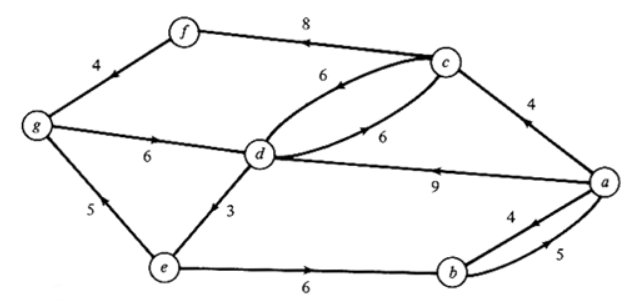
\includegraphics[width=\textwidth]{pcc-mit.png}
        \caption{Digrafo retirado de exercício do site do MIT\cite{mit}}
        \label{konigsberg-graph}
    \end{figure}


    %TODO: Fazer um exemplo pra esse passo a passo, realmente solucionar um caso na mão .


	\begin{thebibliography}{9}
	\bibitem{konigsberg} 
	Euler, Leonhard
	\textit{Solution problematis ad geometriam situs pertinentis}. 
	Comment. Acad. Sci. U. Petrop 8, 128–40, 1736.

	\bibitem{hierholzer}
	Hierholzer, Carl
	\textit{``Über die Möglichkeit, einen Linienzug ohne Wiederholung und ohne Unterbrechung zu umfahren''}, 
	Mathematische Annalen, 6 (1): 30–32, doi:10.1007/BF01442866, 1873.

    \bibitem{sereja}
    Problema retirado do Codeforces, problema C do Round \#215 (Div1)\\
    \href{https://codeforces.com/problemset/problem/367/C}{codeforces.com/problemset/problem/367/C}

    \bibitem{sereja-sol}
    Solução para o problema Sereja and the Arrangement of Numbers, desenvolvida em C++\\
    \href{https://github.com/gafeol/competitive-programming/blob/master/ojs/cf/367/C.cpp}{github.com/gafeol/competitive-programming/blob/master/ojs/cf/367/C.cpp}

    \bibitem{jogging}
    Problema retirado do UVa, problema 10296\\
    \href{https://onlinejudge.org/index.php?option=com_onlinejudge&Itemid=8&page=show_problem&problem=1237}{onlinejudge.org/index.php?option=com\_onlinejudge\&Itemid=8\&page=show\\\_problem\&problem=1237}

    \bibitem{jogging-sol}
    Solução para o problema Jogging Trails, desenvolvida em C++\\
    \href{https://github.com/gafeol/competitive-programming/blob/master/ojs/UVa/1237.cpp}{github.com/gafeol/competitive-programming/blob/master/ojs/UVa/1237.cpp} 

    \bibitem{mit}
    Exemplo retirado do site do MIT, exercício 6.6.c\\
    \href{http://web.mit.edu/urban_or_book/www/book/chapter6/problems6/6.6.html}{web.mit.edu/urban\_or\_book/www/book/chapter6/problems6/6.6.html} 
	\end{thebibliography}
 
\end{document}
